%------------------------------------------------------------------------------------------
% Meta-commands for the TeXworks editor
%
% !TeX root = ../Tesi.tex
% !TEX encoding = UTF-8
% !TEX program = pdflatex
%
\chapter{Flaps, landing gears and spoilers effects on drag}
\label{ch:DeltaCD0FlapSpoiler}
%
\noindent
Flaps, landing gears and spoilers play a key role in the evaluation of the drag of any kind of aircraft during take-off and landing phases. Although very important, these quantities are also very difficult to calculate, especially in a preliminary design phase. This appendix has the purpose of providing to the reader a way to estimate these effects by comparing different possible calculation methods reported on several aircraft design books. 
%
%-----------------------------DELTA CD0 FLAP------------------------------------------
%
\section{$\upDelta C_{D0,\text{flap}}$ calculation methods comparison}\label{par:DeltaCD0FlapComparison}
For the flap contribution to the aircraft drag in take-off and landing, three methods have been compared which uses semi-empirical equations. The first one is from \cite{sforza2014commercial} and provides the following equation.
%
\begin{equation}\label{eq:SforzaCD0}
\upDelta C_{D0}=
    \LEFTRIGHT\lcbrace.{
      \begin{array}{l@{\rule{2em}{0pt}}l} 
        0.9\left(\dfrac{c_f}{c}\right)^{1.38}\left(\dfrac{S_{wf}}{S}\right)\sin^2\delta_f
          & \text{for slotted and fowler flaps}
        \\[1em]
	1.7\left(\dfrac{c_f}{c}\right)^{1.38}\left(\dfrac{S_{wf}}{S}\right)\sin^2\delta_f
          & \text{for plain and split flaps}
      \end{array}
    }  
\end{equation}
%
Using the the flaps input data provided in \ref{par:CaseStudyHighLift} for both the B747-100B and the ATR-72, this method leads to the results of table \ref{tab:SforzaDeltaCD0}.

\bigskip
\noindent
The second method is taken from \cite{nicolai2010fundamentals} and requires to evaluate firstly two constant, $k_1$ and $k_2$, function of $\frac{c_f}{c}$ and $\delta_f$. The values read from these curves are then uses as input for the following equation.
%
\begin{equation}
\upDelta C_{D0}=k_1k_2\dfrac{S_{wf}}{S}
\label{eq:NicolaiCD0}
\end{equation}
%
where $k_1$ and $k_2$ can be read from figures \ref{fig:K1DeltaCD0} and \ref{fig:K2DeltaCD0}. Using the B747-100B and ATR-72 data for high lift devices, it's possible to obtain the results shown in table \ref{tab:NicolaiDeltaCD0}.
%
\clearpage
\vspace*{0.5cm}
%
\begin{table}[H]
  \centering
    \begin{tabular}{c|cc|cc}
    \toprule
    \multicolumn{1}{c}{\textbf{}} & \multicolumn{2}{c}{\textbf{B747-100B}} & \multicolumn{2}{c}{\textbf{ATR-72}} \\
    \midrule
    \multicolumn{1}{c}{\textbf{FLAP 1}} & \multicolumn{1}{c}{\textbf{LND}} & \multicolumn{1}{c}{\textbf{TO}} & \multicolumn{1}{c}{\textbf{LND}} & \multicolumn{1}{c}{\textbf{TO}} \\
    \midrule
    $c_f/c$  & 0.1800 & 0.1800 & 0.3800 & 0.3800 \\
    $\delta_f$ & 30.0000 & 10.0000 & 35.0000 & 20.0000 \\
    $S_{wf}/S$ & 0.4298 & 0.4298 & 0.3463 & 0.3463 \\
    $\upDelta C_{D0,\text{flap}}$ & 0.0091 & 0.0011 & 0.0270 & 0.0096 \\
    \midrule
    \multicolumn{1}{c}{\textbf{FLAP 2}} & \multicolumn{1}{c}{\textbf{LND}} & \multicolumn{1}{c}{\textbf{TO}} & \multicolumn{1}{c}{\textbf{LND}} & \multicolumn{1}{c}{\textbf{TO}} \\
    \midrule
    $c_f/c$  & 0.1800 & 0.1800 & 0.3800 & 0.3800 \\
    $\delta_f$ & 30.0000 & 10.0000 & 35.0000 & 20.0000 \\
    $S_{wf}/S$ & 0.3787 & 0.3787 & 0.5952 & 0.5952 \\
    $\upDelta C_{D0,\text{flap}}$ & 0.0080 & 0.0010 & 0.0464 & 0.0165 \\
    \midrule
    \midrule
    \multicolumn{1}{c}{\textbf{TOTAL}} & \multicolumn{1}{c}{\textbf{LND}} & \multicolumn{1}{c}{\textbf{TO}} & \multicolumn{1}{c}{\textbf{LND}} & \multicolumn{1}{c}{\textbf{TO}} \\
    \midrule
    \textbf{$\upDelta C_{D0,\text{flap}}$} & \textbf{0.0171} & \textbf{0.0021} & \textbf{0.0733} & \textbf{0.0261} \\
    \bottomrule
    \end{tabular}
    \caption{$\upDelta C_{D0,\text{flap}}$ calculation using equation \ref{eq:SforzaCD0} for the B747-100B and the ATR-72}
    \label{tab:SforzaDeltaCD0}
\end{table}
%
\vspace*{1.5cm}
%
\begin{table}[H]
  \centering
    \begin{tabular}{c|cc|cc}
    \toprule
    \multicolumn{1}{c}{\textbf{}} & \multicolumn{2}{c}{\textbf{B747-100B}} & \multicolumn{2}{c}{\textbf{ATR-72}} \\
    \midrule
    \multicolumn{1}{c}{\textbf{FLAP 1}} & \multicolumn{1}{c}{\textbf{LND}} & \multicolumn{1}{c}{\textbf{TO}} & \multicolumn{1}{c}{\textbf{LND}} & \multicolumn{1}{c}{\textbf{TO}} \\
    \midrule
    $c_f/c$  & 0.1800 & 0.1800 & 0.3800 & 0.3800 \\
    $k_1$    & 0.8968 & 0.8968 & 2.6353 & 2.6353 \\
    $t/c$   & 0.1300 & 0.1300 & 0.1670 & 0.1670 \\
    $k_2$    & 0.0206 & 0.0031 & 0.0284 & 0.0085 \\
    $S_{wf}/S$ & 0.4298 & 0.4298 & 0.3463 & 0.3463 \\
    $\upDelta C_{D0,\text{flap}}$ & 0.0080 & 0.0012 & 0.0259 & 0.0077 \\
    \midrule
    \multicolumn{1}{c}{\textbf{FLAP 2}} & \multicolumn{1}{c}{\textbf{LND}} & \multicolumn{1}{c}{\textbf{TO}} & \multicolumn{1}{c}{\textbf{LND}} & \multicolumn{1}{c}{\textbf{TO}} \\
    \midrule
    $c_f/c$  & 0.1800 & 0.1800 & 0.3800 & 0.3800 \\
    $k_1$    & 0.8968 & 0.8968 & 2.6353 & 2.6353 \\
    $t/c$   & 0.1300 & 0.1300 & 0.1670 & 0.1670 \\
    $k_2$    & 0.0206 & 0.0031 & 0.0284 & 0.0085 \\
    $S_{wf}/S$ & 0.3787 & 0.3787 & 0.5952 & 0.5952 \\
    $\upDelta C_{D0,\text{flap}}$ & 0.0070 & 0.0011 & 0.0445 & 0.0133 \\
    \midrule
    \midrule
    \multicolumn{1}{c}{\textbf{TOTAL}} & \multicolumn{1}{c}{\textbf{LND}} & \multicolumn{1}{c}{\textbf{TO}} & \multicolumn{1}{c}{\textbf{LND}} & \multicolumn{1}{c}{\textbf{TO}} \\
    \midrule
    \textbf{$\upDelta C_{D0,\text{flap}}$} & \textbf{0.0150} & \textbf{0.0023} & \textbf{0.0704} & \textbf{0.0211} \\
    \bottomrule
    \end{tabular}
    \caption{$\upDelta C_{D0,\text{flap}}$ calculation using equation \ref{eq:NicolaiCD0} for the B747-100B and the ATR-72}
  \label{tab:NicolaiDeltaCD0}
\end{table}
%
\begin{figure}[H]
\centering
\includegraphics[width=\linewidth]{K1_Nicolai.PNG}
\caption{The functions $k_1\left(c_f/c\right)$ all type of flaps}
\label{fig:K1DeltaCD0}
\end{figure}
%
\begin{figure}[H]
\centering
\includegraphics[width=\linewidth]{K2_Nicolai.PNG}
\caption{The functions $k_2\left(\delta_f\right)$ all type of flaps}
\label{fig:K2DeltaCD0}
\end{figure}
%
\noindent
The last method used is the one proposed in \cite{Young:Flaps} and described in the subsection \ref{subpar:DCD0}. It uses the following equation in which $\delta_1$ and $\delta_2$ can be evaluated using the charts in figures \ref{fig:K1DeltaCD0} and \ref{fig:K2DeltaCD0}; while $\delta_3$ can be read from the chart of figure \ref{fig:Delta3}. Table \ref{tab:YoungDeltaCD0} resume the results obtained using this method with the flap data of the B747-100B and of the ATR-72.
%
\begin{equation}
\upDelta C_{D0}=\delta_1\left(c_f/c\right)\delta_2\left(\delta_f\right)\delta_3\left(b_f/b\right)
\label{eqn:DeltaCD0PartSpan}
\end{equation}
%
\begin{figure}[H]
\centering
\includegraphics[width=0.77\linewidth]{Delta3}
\caption{The functions $\delta_3\left(b_f/b\right)$ for slotted flaps}
\label{fig:Delta3}
\end{figure}
%
\begin{table}[H]
  \centering
    \begin{tabular}{c|cc|cc}
    \toprule
    \multicolumn{1}{c}{\textbf{}} & \multicolumn{2}{c}{\textbf{B747-100B}} & \multicolumn{2}{c}{\textbf{ATR-72}} \\
    \midrule
    \multicolumn{1}{c}{\textbf{FLAP 1}} & \multicolumn{1}{c}{\textbf{LND}} & \multicolumn{1}{c}{\textbf{TO}} & \multicolumn{1}{c}{\textbf{LND}} & \multicolumn{1}{c}{\textbf{TO}} \\
    \midrule
    $c_f/c$  & 0.1800 & 0.1800 & 0.3800 & 0.3800 \\
    $k_1$    & 0.8968 & 0.8968 & 2.6353 & 2.6353 \\
    $t/c$   & 0.1300 & 0.1300 & 0.1670 & 0.1670 \\
    $k_2$    & 0.0206 & 0.0031 & 0.0284 & 0.0085 \\
    Taper ratio & 0.2650 & 0.2650 & 0.5450 & 0.5450 \\
    $b_f/b$  & 0.2710 & 0.2710 & 0.2700 & 0.2700 \\
    $k_3$    & 0.3521 & 0.3521 & 0.3033 & 0.3033 \\
    $\upDelta C_{D0,\text{flap}}$ & 0.0065 & 0.0010 & 0.0227 & 0.0068 \\
    \midrule
    \multicolumn{1}{c}{\textbf{FLAP 2}} & \multicolumn{1}{c}{\textbf{LND}} & \multicolumn{1}{c}{\textbf{TO}} & \multicolumn{1}{c}{\textbf{LND}} & \multicolumn{1}{c}{\textbf{TO}} \\
    \midrule
    $c_f/c$  & 0.1800 & 0.1800 & 0.3800 & 0.3800 \\
    $k_1$    & 0.8968 & 0.8968 & 2.6353 & 2.6353 \\
    $t/c$   & 0.1300 & 0.1300 & 0.1670 & 0.1670 \\
    $k_2$    & 0.0206 & 0.0031 & 0.0284 & 0.0085 \\
    Taper Ratio & 0.2650 & 0.2650 & 0.5450 & 0.5450 \\
    $b_f/b$  & 0.2250 & 0.2250 & 0.4500 & 0.4500 \\
    $k_3$    & 0.3154 & 0.3154 & 0.5034 & 0.5034 \\
    $\upDelta C_{D0,\text{flap}}$ & 0.0058 & 0.0009 & 0.0376 & 0.0113 \\
    \midrule
    \multicolumn{1}{c}{\textbf{TOTAL}} & \multicolumn{1}{c}{\textbf{LND}} & \multicolumn{1}{c}{\textbf{TO}} & \multicolumn{1}{c}{\textbf{LND}} & \multicolumn{1}{c}{\textbf{TO}} \\
    \midrule
    \textbf{$\upDelta C_{D0,\text{flap}}$} & \textbf{0.0124} & \textbf{0.0019} & \textbf{0.0603} & \textbf{0.0181} \\
    \bottomrule
    \end{tabular}
        \caption{$\upDelta C_{D0,\text{flap}}$ calculation using equation \ref{eq:NicolaiCD0} for the B747-100B and the ATR-72}
  \label{tab:YoungDeltaCD0}
\end{table}
%
\noindent
From the three analysis performed, a good value of  $\upDelta C_{D0,\text{flap}}$ can be taken from the following table both in take-off or landing configuration; in particular for the take-off and landing analysis of chapter \ref{chap:TakeOff} the value derived from Young\cite{Young:Flaps} has been considered. 
%
\begin{table}[htbp]
  \centering
    \begin{tabular}{ccc||ccc}
    \toprule
    \multicolumn{3}{c}{\textbf{Method Comparison B747-100B}} & \multicolumn{3}{c}{\textbf{Method Comparison ATR-72}} \\
    \midrule
          & \multicolumn{1}{c}{\textbf{TO}} & \multicolumn{1}{c}{\textbf{LND}} &       & \multicolumn{1}{c}{\textbf{TO}} & \multicolumn{1}{c}{\textbf{LND}} \\
          \midrule
    \multicolumn{1}{c}{\textbf{SFORZA}} & 0.0021 & 0.0171 & \multicolumn{1}{c}{\textbf{SFORZA}} & 0.0261 & 0.0733 \\
    \multicolumn{1}{c}{\textbf{NICOLAI}} & 0.0023 & 0.0150 & \multicolumn{1}{c}{\textbf{NICOLAI}} & 0.0211 & 0.0704 \\
    \multicolumn{1}{c}{\textbf{YOUNG}} & 0.0019 & 0.0124 & \multicolumn{1}{c}{\textbf{YOUNG}} & 0.0181 & 0.0603 \\
    \bottomrule
    \end{tabular}
    \caption{Summary of $\upDelta C_{D0,\text{flap}}$ obtained for the B747-100B and for the ATR-72 in take-off and landing configuration}
\end{table}
%
%-----------------------------DELTA CD0 LANDING GEARS------------------------------------------
%
\section{$\upDelta C_{D0,\text{landing gear}}$ evaluation}\label{par:DeltaCD0LGComparison}
The value of $\upDelta C_{D0,\text{landing gear}}$ can be one of the most difficult parameter to be estimated in a preliminary design phase; in fact, it requires that the landing gear itself has, at least, been sized so that the drag coefficient could be estimated through it's equivalent parasite area. When all this information are not available, a good way to estimate this parameter can be a statistical approach like the one proposed by \cite{nicolai2010fundamentals} and represented in the following chart.
%
\begin{figure}[H]
\centering
\includegraphics[width=0.85\linewidth]{LandingGearNicolai.PNG}
\caption{$\upDelta C_{D0,\text{landing gear}}$ as function of $\delta_{\text{flap}}$ for several aircraft categories}
\end{figure}
%
\noindent
As can be seen the value of $\upDelta C_{D0,\text{landing gear}}$ is not precise but can be chosen among several values suitable for that aircraft category; furthermore, it is important to highlight the effect of flaps deflection which reduces the landing gear contribution to the parasite drag when the deflection grows.
%
%----------------------------------DELTA CD0 SPOILERS--------------------------------------------
%
\section{$\upDelta C_{D0,\text{spoiler}}$ calculation methods comparison}\label{par:DeltaCD0SpoilerComparison}
Spoilers effects on drag are present only in landing configuration and determine big increment of the drag coefficient of the aircraft during the approach and landing phase. This increment can be estimated knowing the spoilers area and the aircraft wing geometry. In this section two way of calculating these effects are shown; one is proposed in \cite{roskamAirplane} while the second is from~\cite{Lausetti:decollo}.

\bigskip
\noindent
The first one considers the $\upDelta C_{D0,\text{spoiler}}$ as function only of the spoiler type (solid plate on wing, flat plate on fuselage, etc.) and of the spoiler surface to wing surface ratio $\frac{S_{sp}}{S}$; this leads to the following equation.
%
\begin{equation}
\upDelta C_{D0,\text{spoiler}}=\sum_{i=0}^n \upDelta C_{Dsp,i}\ \dfrac{S_{sp,i}}{S}
\label{eqn:RoskamSpoiler}
\end{equation}
%
\noindent
where $\upDelta C_{Dsp,i}$ is related to the spoiler type as shown in the following figure.
%
\begin{figure}[H]
\centering
\includegraphics[width=0.9\linewidth]{Roskam_Spoiler.pdf}
\caption{$\upDelta C_{Dsp,i}$ as function of the spoiler type}
\label{fig:SpoilerType}
\end{figure}

\bigskip
\noindent
This method applied for the B747-100B, whose spoilers are of the second type of figure \ref{fig:SpoilerType}, and for the ATR-72, whose two spoilers are mounted on the top of the fuselage, leads to the following results. 
%
\clearpage
%
\begin{table}[!t]
  \centering
  \scalebox{0.9}{
    \begin{tabular}{l||cc}
    \toprule
          & \textbf{B747-100B} & \textbf{ATR-72} \\
    \midrule
    \textbf{SPOILER 1} & & \\
    \midrule
    \textbf{$S_{sp}/S$} & 0.029 & 0.055 \\
    \textbf{$\upDelta C_{Dsp,i}$} & 1.6   & 1.0 \\
    \midrule
    \textbf{SPOILER 2} & & \\
    \midrule
    \textbf{$S_{sp}/S$} & 0.026 & 0.055 \\
    \textbf{$\upDelta C_{Dsp,i}$} & 1.6   & 1.0 \\
    \midrule
    \midrule
    \textbf{TOTAL} & & \\
    \midrule
    \textbf{$\upDelta C_{D\text{spoiler}}$} & 0.088 & 0.011 \\
    \bottomrule
    \end{tabular}
    }
    \caption{$\upDelta C_{D0,\text{spoiler}}$ of B747-100B and ATR-72 using equation \ref{eqn:RoskamSpoiler}}
\end{table}
%
\noindent
The second method considers the $\upDelta C_{D0,\text{spoiler}}$ as function of the spoiler surface to wing surface ratio $\frac{S_{sp}}{S}$ and also of the following parameters.
%
\begin{itemize}
\item The drag coefficient related to the spoiler surface, $C_{D\text{local}}$.
\item The interference factor $\phi=\left(\frac{V'}{V}\right)^2$, which takes into account of the wing interference with the spoiler and can estimated from the chart in figure \ref{fig:InterferenceSpoiler}.
\item The leading edge sweep angle of the wing, $\Lambda$.
\item The spoiler aspect ratio, $\lambda=\frac{b}{a}$
\end{itemize}
%
\begin{equation}
\upDelta C_{D0,\text{spoiler}}=\phi\cdot C_{D\text{local}}\cdot \dfrac{S_{sp}}{S}\cdot \left[\cos^{\frac{3}{2}}\left(\Lambda\right)+K_\delta\cos^2 \left(2\Lambda\right)\right]
\label{eqn:LausettiSpoiler}
\end{equation}
%
\noindent
where $K_\delta$ is function of the spoiler aspect ratio $\lambda$ as shown below.
%
\begin{equation}
K_\delta=0.25\cdot\left[\dfrac{\left(\lambda-1\right)}{\lambda}\right]^{\frac{1}{2}}
\end{equation}
%
\noindent
This method is suitable only for those spoilers mounted on the wing, so that the results shown will concern only the B747-100B.
%
\begin{table}[H]
  \centering
\scalebox{0.9}{
    \begin{tabular}{lr|lr}
    \toprule
    \multicolumn{4}{c}{\textbf{B747-100B}} \\
    \midrule
    \textbf{Spoiler 1} &  & \textbf{Spoiler 2} & \\
    \midrule
    \textbf{$S_{sp}/S$} & 0.029 & \textbf{$S_{sp}/S$} & 0.026  \\
    \textbf{$\phi$} & 1.44 & \textbf{$\phi$} & 1.44 \\
    \textbf{$C_{D\text{local}}$} & 1.28 & \textbf{$C_{D\text{local}}$} & 1.12 \\
    \textbf{$\lambda$} & 7.6 &  \textbf{$\lambda$} & 6.3 \\
    \textbf{$K_\delta$} & 0.233 & \textbf{$K_\delta$} & 0.161 \\
    \textbf{$\Lambda$} & $\SI{37}{\degree}$ &  \textbf{$\Lambda$} & $\SI{37}{\degree}$ \\
    \textbf{$\upDelta C_{D\text{spoiler}}$} & 0.0391 &  \textbf{$\upDelta C_{D\text{spoiler}}$} & 0.0304 \\
    \midrule
    \midrule
     \multicolumn{4}{c}{\textbf{Total}} \\
    \midrule
     \multicolumn{2}{c}{\textbf{$\upDelta C_{D\text{spoiler}}$}} &  \multicolumn{2}{c}{0.0695} \\
    \bottomrule
    \end{tabular}
    }
      \caption{$\upDelta C_{D0,\text{spoiler}}$ of B747-100B and ATR-72 using equation \ref{eqn:LausettiSpoiler}}
\end{table}

%
\begin{figure}[H]
\centering
\includegraphics[width=0.7\linewidth]{V'V}
\caption{Speed distribution on the the upper and lower surface of an airfoil}
\label{fig:InterferenceSpoiler}
\end{figure}
%